% !TEX root = ../my-thesis.tex
%
\chapter{Appendix}
\label{sec:appendix}

\section{Drone surveys processing methodology}
\label{sec:drone_method}

\begin{table}
  \centering
  \caption{List of all the studied AIRs in Ladakh.}
	\label{tab:Ladakh_AIRs}
	\begin{tabular}{|lllll|}
    \hline
    \textbf{Location}     & \textbf{Winter season} & \textbf{Altitude [$m\,a.s.l.$]} & \textbf{
    Radius [$m$]} & \textbf{Volume [$m^3$]} \\ \hline
    Igoo & 2019--20 & 4209 & 23 & 4918  \\
    Karith & 2019--20 & 3710 & 12 & 1451  \\
    Karith 2 & 2020--21 & 3692 & 5 & 1133  \\
    Lamso & 2019--20 & 3859 & 7 & 615  \\
    Lamso 2& 2020--21 & 3863 & 6 & 420  \\
    Nang& 2019--20 & 3897 & 13 & 1601 \\
    Phyang& 2019--20 & 3916 & 19 & 5182 \\
    Sandoo& 2019--20 & 3773 & 10 & 1483 \\
    Shara& 2019--20 & 4288 & 18 & 7936 \\
    Gangles& 2020--21 & 4072 & 9 & 602 \\
    Apati& 2020--21 & 3840 & 6 & 351 \\
    Mulbeck& 2019--20 & 3451 & 11 & 1887\\
    Nang& 2019--20 & 3897 & 13 & 1601\\
    Skurbuchan& 2019--20 & 3023 & 9 & 956\\
    Takmachik& 2019--20 & 3032 & 13 &1265\\
    Takmachik 2& 2020--21 & 3052 & 10 &1604\\
    Tarchit& 2020--21 & 3962 & 17 &2363\\
    Patherak& 2020--21 & 3899 & 10 &770\\
    Kullum& 2020--21 & 3907 & 7 &328\\ \hline
	\end{tabular}
\end{table}

\begin{figure}
	\begin{center}
		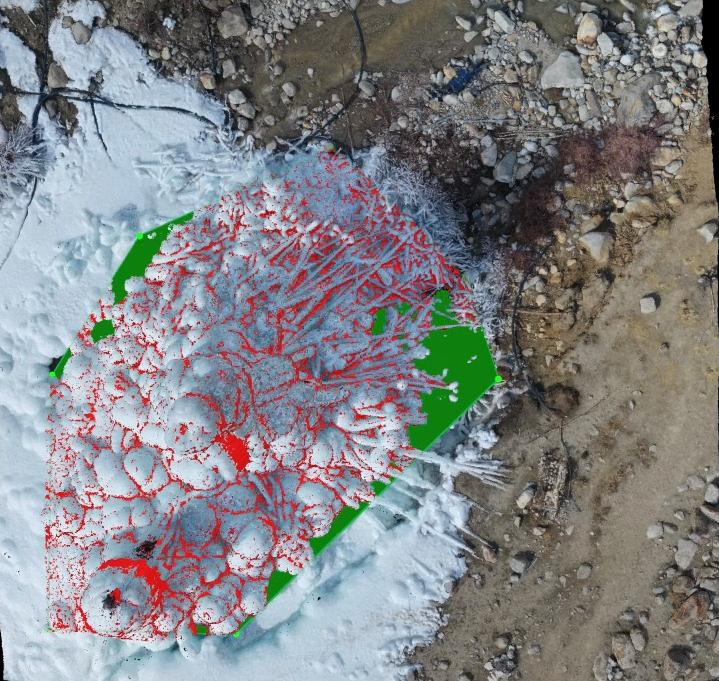
\includegraphics[width=12 cm]{figs/pix4d.jpg}
	\end{center}
	\caption{Digital elevation map of Indian AIR constructed from the drone survey on March 3, 2021. The green
		area represents the area bounded by the marked perimeter and the red area represents gaps in the point cloud
    that were filled to compute the associated volume.
	}
	\label{fig:DEM}
\end{figure}

The drone flew along a predefined flight course and took photographs at a set time interval. The
position and altitude of the drone at the exposure stations, which were obtained by the built-in integrated
Position and Orientation System (POS, composed of a global positioning system and inertial measurement units),
were recorded in JPEG pictures. In this study, we adopted a three-step workflow as implemented in the
commercial software package Pix4Dmapper version 4.6.4 (\cite{pix4dsaPix4DmapperUserManual2020}). A short summary of this workflow is
described below:

(1) Initial processing: This process generates a sparse point cloud with the structure-from motion algorithm
(\cite{turnerAutomatedTechniqueGenerating2012}). First, it searches for and matches key points in the photos that have certain overlapping
areas using a feature matching algorithm (e.g., the scale-invariant feature transform (SIFT) algorithm, which can
detect key points in photos with different views and illumination conditions;
\cite{loweDistinctiveImageFeatures2004}). Second, the approximate locations and orientations of the camera at
each exposure station are reconstructed with the internal parameters (focal length, coordinates of the principal
point of the photograph), and external parameters (i.e. POS data). A sparse point cloud is created.

(2) Point cloud densification: In this step, the multi-view stereo technique is applied to achieve a higher
point cloud density than in the previous step (\cite{furukawaAccurateDenseRobust2010};
\cite{molgStructurefromMotionUsingHistorical2017}). Thus, the spatial resolution of the products can be
increased, and an irregular network for the next step can be created (\cite{kungACCURACYAUTOMATICPHOTOGRAMMETRIC2011}).

(3) AIR delineation: Ice radius, area and volume are the three final products. Perimeter was manually marked
on the point cloud by identifying the AIR boundary (see Fig. \ref{fig:DEM}). For the Indian location, we identified identical rock features
near the ice boundary to mark as vertices of this perimeter. For the Swiss AIR, no such feature was available due
to snowfall, so instead the perimeter was marked by identifying the ice and snow boundary.

There is temporal and spatial uncertainty associated with this process. Weather conditions influence the quality
of each drone survey to various degrees. Moreover, since ice/snow surfaces do not have many identifiable features, few
feature points can be detected and matched in the vicinity of the AIR. Thus, we attach a high uncertainty of
$\pm 10 \%$ for all the AIR observations to accommodate for this.

\section{Sensitivity and uncertainty analysis} \label{sec:uncertainpy}

In this section, we summarise the theory behind the methods for uncertainty quantification and sensitivity
analysis used. For a detailed explanation of this methodology, see \cite{tennoeUncertainpyPythonToolbox2018}.

\subsection{Problem definition}
Consider our model $U$ that depends on timestep $i$, has $d$ uncertain parameters $Q = [Q_1, Q_2, \dots, Q_d]$, and
gives output $V_{ice}$:

\begin{equation}
V_{ice} = U(i,Q)
\end{equation}

The output $V_{ice}$ can have any value within the output space and has an unknown probability density function
$\rho_{V_{ice}}$. The goal of our uncertainty quantification is to describe the unknown $\rho_{V_{ice}}$ through
statistical metrics.

We assume that all these parameters are statistically independent from each other and have a uniform probability
density function $\rho_{Q_j}$. The joint multivariate probability density function for the uncertain parameters
is then:

\begin{equation}
\rho_{Q} = \prod_{j = 1}^{d} \rho_{Q_j}
\end{equation}

As mentioned, the goal of an uncertainty quantification is to describe the unknown distribution of the model
output through statistical metrics. A useful metric is the $(100 \cdot x)$-th percentile $P_x$ of $V_{ice}$,
which defines a value below  which $100 \cdot x$ percent of the model outputs are located. We can combine two
percentiles to create a prediction interval, which is a range of values within which a $100 \cdot x$
percentage of the outputs $V_{ice}$ occur. In our methodology, we use the 90 \% prediction interval $I^k$, as
the metric to compare the uncertainties of a given set of parameters $Q^k$. This is defined as:  

\begin{equation}
I^k = [P_{(0.9/2)}, P_{(1-0.9/2)}]
\end{equation}

\subsection{Sensitivity analysis}

We use a variance-based sensitivity analysis and compute the commonly considered Sobol sensitivity indices
(Sobol, 1990). The Sobol sensitivity indices quantify how much of the variance in the model output each
uncertain parameter is responsible for. There are several types of Sobol indices. The first order Sobol
sensitivity index $S_j$ measures the direct effect each parameter has on the variance of the model. Higher order
Sobol indices give the sensitivity due to interactions between a parameter $Q_j$ and various other parameters.
The total Sobol sensitivity $S_{T_{j}}$ includes the sensitivity of both first order effects, as well as the
sensitivity due to interactions between a given parameter $Q_j$ and all combinations of the other
parameters. The sum of the total Sobol sensitivity indices is equal to or greater than one, and is only equal to
one if there are no interactions between the parameters. Our goal is to use sensitivity analysis to fix
parameters with high sensitivity, so the total-order Sobol indices are an appropriate metric.

\subsection{Polynomial Chaos Expansions}

A recent mathematical framework for efficient uncertainty quantification and sensitivity analysis is that of
polynomial chaos expansions (\cite{xiuHighOrderCollocationMethods2005}). This method calculates the same statistical metrics as the Monte
Carlo method but typically much faster.

The general idea behind polynomial chaos expansions is to approximate the model $U$ with a polynomial expansion
$\hat{U}$ : 

\begin{equation} U \approx \hat{U}(i, Q) = \sum_{n=0}^{N_p-1} c_n(i) \phi_n(Q) \end{equation}

where $\phi_n$ are polynomials, and $c_n$ are expansion coefficients. The number of expansion factors $N_p$ is
given by

\begin{equation}
  N_p = \binom{d+p}{p}
\end{equation}

where $p$ is the polynomial order. 

The first and total-order indices can also be calculated directly from the polynomial chaos expansion. On the
other hand, the $90\, \%$ prediction interval ($I$) must be estimated by using $\hat{U}$ as a surrogate
model.

\section{Model forcing based on water-use efficiency and maximum ice volume objectives}
\label{sec:auto_software}

The model complexity and data requirement (paper I) were reduced through assumptions that optimise for the ice
volume or the water-use efficiency objectives. The corresponding model assumptions are called IVOM and WEOM
respectively. We define the freezing rate and melting rate as the positive and negative mass change rate,
respectively. Assumptions are chosen, based on whether they overestimate/underestimate the freezing rate. IVOM
assumptions overestimates freezing rate whereas WEOM assumptions underestimates freezing rate. We describe these
two kinds of assumptions applied on each of the energy balance components below: 

\subsection{Surface Area $A_{cone}$ assumptions}

The surface area during the accumulation period is determined by assuming a constant ice cone
radius equal to the fountain spray radius. The surface area scales the freezing rate of the AIR. Hence, for the
IVOM version, we assume the maximum possible slope of 1 for the ice cone or in other words $h_{cone} = r_{F}$.
Therefore, area is estimated as:  

\begin{equation} A_{cone} =\sqrt{2} \cdot \pi \cdot r_{F}^2  \end{equation}

Similarly, for the water-use efficiency objective, the area of the conical AIR is approximated to the area of
its circular base. Therefore, area is estimated as:

\begin{equation} A_{cone} =\pi \cdot r_{F}^2  \end{equation}

\subsection{Net shortwave radiation \texorpdfstring{$q_{SW}$}{Lg} assumptions}

The net shortwave radiation $q_{SW}$ is computed as follows:

\begin{equation} 
q_{SW} = (1- \alpha) \cdot ( SW_{direct} \cdot f_{cone} + SW_{diffuse})
\end{equation}

where $\alpha$ is the albedo value ; $SW_{direct}$ is the direct shortwave radiation; $SW_{diffuse}$ is the
diffuse shortwave radiation and $f_{cone}$ is the solar area fraction.

The data requirement was reduced by estimating the global shortwave radiation and pressure directly using the
location's coordinates and altitude through the solar radiation model described in
\citet{holmgrenPvlibPythonPython2018}. The algorithm used to estimate the clear-sky global radiation is
described in \citet{ineichenBroadbandSimplifiedVersion2008}.  

The diffuse and direct shortwave radiation is determined using the estimated global solar radiation as follows:

\begin{equation}
\begin{split}
  SW_{diffuse} &= cld \cdot SW_{global}\\
  SW_{direct} &= (1-cld) \cdot SW_{global}
\end{split}
\end{equation}

where $cld$ is the cloudiness factor. $cld$ is assumed to be 1 and 0 for the water-use efficiency and ice volume
objective respectively.

We ignore the variations in the albedo and assume it to be equal to snow albedo and ice albedo for the  ice
volume and water-use efficiency objective, respectively.

The solar area fraction $f_{cone}$ of the ice structure exposed to the direct shortwave radiation depends on the
shape considered. It is computed as

\begin{equation}
		f_{cone} =\frac{(0.5 \cdot r_{cone} \cdot h_{cone}) \cdot cos \theta_{sun} +(\pi \cdot
			{(r_{cone})}^2/2) \cdot sin \theta_{sun} }{\pi \cdot r_{cone} \cdot ({(r_{cone})}^2+{(h_{cone})}^2)^{1/2}}\\
\end{equation}

For the ice volume objective, since we assume the slope of the cone to be 1, $f_{cone}$ is determined as follows:

\begin{equation}
		f_{cone} =\frac{ cos \theta_{sun} + \pi \cdot sin \theta_{sun} }{2\sqrt{2} \cdot \pi }
\end{equation}

Similarly, for the water-use efficiency objective, since we assume the slope of the cone to be negligible, we get:

\begin{equation}
		f_{cone} =\frac{ sin \theta_{sun} }{2 }
\end{equation}

\subsection{Net Longwave radiation \texorpdfstring{$q_{LW}$}{Lg} assumptions} 

We assume $T_{ice} = 0 \degree C$ in order to determine outgoing longwave radiation. Since it is challenging to
constrain the minimum ice temperature, we maintain this assumption for both our objectives. However, in order to
estimate atmospheric emissivity, we again assume $cld$ to be 1 and 0 for the water-use efficiency and ice volume
objective respectively.

\subsection{Turbulent fluxes assumptions} 

Turbulent fluxes estimation depend on the slope of the cone through the $\mu_{cone}$ parameter. As suggested 
by \citet{oerlemansBriefCommunicationGrowth2021}, we estimated this parameter as follows:

\begin{equation}
  \mu_{cone} =1 + s_{cone}/2
\end{equation}

Hence, the $\mu_{cone}$ parameter takes values of 1.5 and 1 for the ice volume and water-use efficiency
objective respectively.  Since turbulent fluxes impact both the freezing and the melting rates, this assumption
may not favor the corresponding objectives for certain sites.

% \section{Quantification of the adaptation potential of Stok catchment}\label{sec:adaptation}

% Stok catchment in Ladakh is fed by a glacier with area of 0.8 $km^2$ (1969) and has a dry season melt rate of
% 0.25 $mm/day$ \cite{sohebMassbalanceObservationReconstruction2020}. This implies the village receives around
% 0.002 $m^3/s$ of glacial meltwater supply during April and May. Icestupa meltwater quantities measured in nearby
% villages supply more than 10 $m^3/day$ (Fig.\ref{fig:ISmelt}) or about 10 percent of Stok's glacial water supply.
% Therefore, to adapt against 8 \% reduction in glacial meltwater supply only 1 ice stupa is required.

% \section{Appendix Section 2}
% \label{sec:appendix:sec2}

% \Blindtext[1][1]

% \begin{table}[h]
% 	\begin{tabularx}{\textwidth}{X | X | X}
% 		%\hline
% 		Alpha		& Beta			& Gamma			\\ \hline
% 		0			& 1				& 2				\\ \hline
% 		3			& 4				& 5				\\ %\hline
% 	\end{tabularx}
% 	\label{tab:table2}
% 	\caption{This is a caption text.}
% \end{table}

% \Blindtext[1][2]
